
\documentclass{article}\usepackage[]{graphicx}\usepackage[]{color}
%% maxwidth is the original width if it is less than linewidth
%% otherwise use linewidth (to make sure the graphics do not exceed the margin)
\makeatletter
\def\maxwidth{ %
  \ifdim\Gin@nat@width>\linewidth
    \linewidth
  \else
    \Gin@nat@width
  \fi
}
\makeatother

\definecolor{fgcolor}{rgb}{0.345, 0.345, 0.345}
\newcommand{\hlnum}[1]{\textcolor[rgb]{0.686,0.059,0.569}{#1}}%
\newcommand{\hlstr}[1]{\textcolor[rgb]{0.192,0.494,0.8}{#1}}%
\newcommand{\hlcom}[1]{\textcolor[rgb]{0.678,0.584,0.686}{\textit{#1}}}%
\newcommand{\hlopt}[1]{\textcolor[rgb]{0,0,0}{#1}}%
\newcommand{\hlstd}[1]{\textcolor[rgb]{0.345,0.345,0.345}{#1}}%
\newcommand{\hlkwa}[1]{\textcolor[rgb]{0.161,0.373,0.58}{\textbf{#1}}}%
\newcommand{\hlkwb}[1]{\textcolor[rgb]{0.69,0.353,0.396}{#1}}%
\newcommand{\hlkwc}[1]{\textcolor[rgb]{0.333,0.667,0.333}{#1}}%
\newcommand{\hlkwd}[1]{\textcolor[rgb]{0.737,0.353,0.396}{\textbf{#1}}}%
\let\hlipl\hlkwb

\usepackage{framed}
\makeatletter
\newenvironment{kframe}{%
 \def\at@end@of@kframe{}%
 \ifinner\ifhmode%
  \def\at@end@of@kframe{\end{minipage}}%
  \begin{minipage}{\columnwidth}%
 \fi\fi%
 \def\FrameCommand##1{\hskip\@totalleftmargin \hskip-\fboxsep
 \colorbox{shadecolor}{##1}\hskip-\fboxsep
     % There is no \\@totalrightmargin, so:
     \hskip-\linewidth \hskip-\@totalleftmargin \hskip\columnwidth}%
 \MakeFramed {\advance\hsize-\width
   \@totalleftmargin\z@ \linewidth\hsize
   \@setminipage}}%
 {\par\unskip\endMakeFramed%
 \at@end@of@kframe}
\makeatother

\definecolor{shadecolor}{rgb}{.97, .97, .97}
\definecolor{messagecolor}{rgb}{0, 0, 0}
\definecolor{warningcolor}{rgb}{1, 0, 1}
\definecolor{errorcolor}{rgb}{1, 0, 0}
\newenvironment{knitrout}{}{} % an empty environment to be redefined in TeX

\usepackage{alltt}
\usepackage[margin=1in]{geometry}
\usepackage{float}
\usepackage{subcaption}
\usepackage{amssymb,amsmath,amsfonts}
\usepackage[multiple]{footmisc}
\usepackage[utf8]{inputenc}
\usepackage{pdflscape}
\usepackage{booktabs}
\usepackage{ctable}
\usepackage{thumbpdf}
\IfFileExists{upquote.sty}{\usepackage{upquote}}{}
\begin{document}




\subsection{Proof-of-concept simulation. Simulation scenario 1 with 3 time-points.}

\begin{knitrout}
\definecolor{shadecolor}{rgb}{0.969, 0.969, 0.969}\color{fgcolor}\begin{kframe}
\begin{alltt}
\hlkwd{load}\hlstd{(}\hlstr{"/Users/olegsofrygin/GoogleDrive/Alex_SDR/sims/sims_final_04_20_17/sim1_results_t2.Rd"}\hlstd{)}
\hlkwd{print}\hlstd{(results[[}\hlstr{"res_name"}\hlstd{]])}
\end{alltt}
\begin{verbatim}
## [1] "results for E[Y_d(t)] for \bar{A}=1, t=2, N = 500, nsims = 1000"
\end{verbatim}
\end{kframe}
\end{knitrout}

\begin{knitrout}
\definecolor{shadecolor}{rgb}{0.969, 0.969, 0.969}\color{fgcolor}\begin{figure}[H]

{\centering 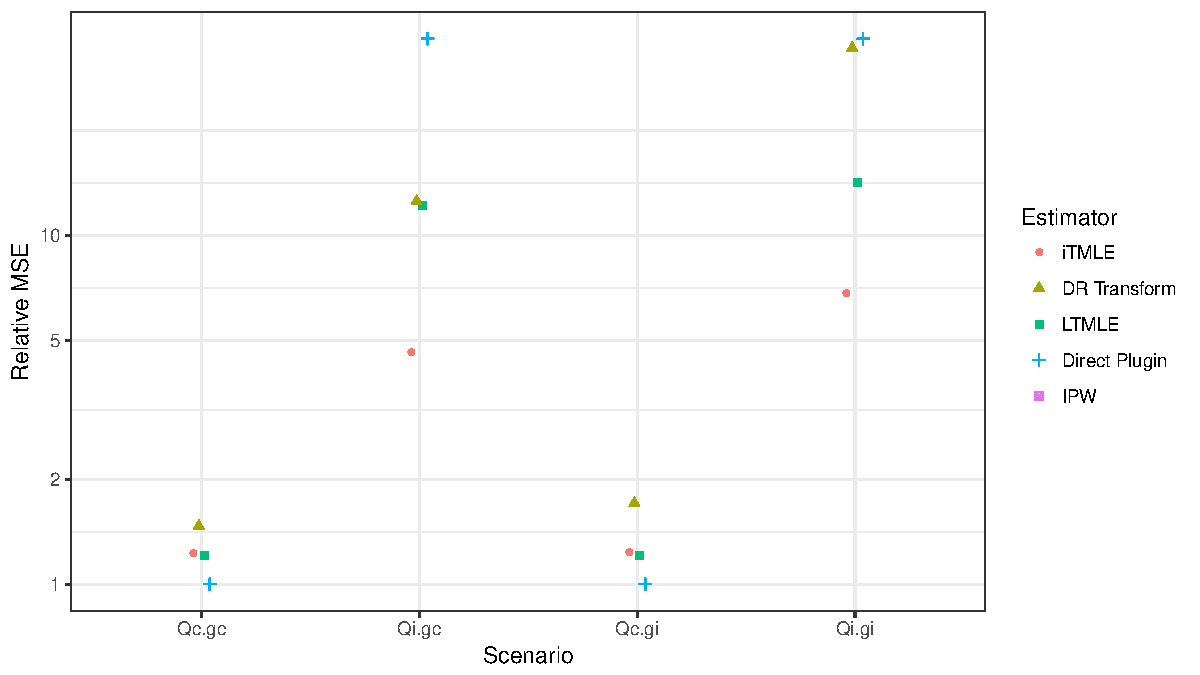
\includegraphics[width=.7\linewidth]{figure/plot-ggplot_MSE_t3-1} 

}

\caption[Relative MSE for $\hat{Q}_1$ in simulation scenario 1 with 3 time points]{Relative MSE for $\hat{Q}_1$ in simulation scenario 1 with 3 time points.}\label{fig:ggplot.MSE.t3}
\end{figure}


\end{knitrout}

\begin{knitrout}
\definecolor{shadecolor}{rgb}{0.969, 0.969, 0.969}\color{fgcolor}\begin{figure}[H]

{\centering 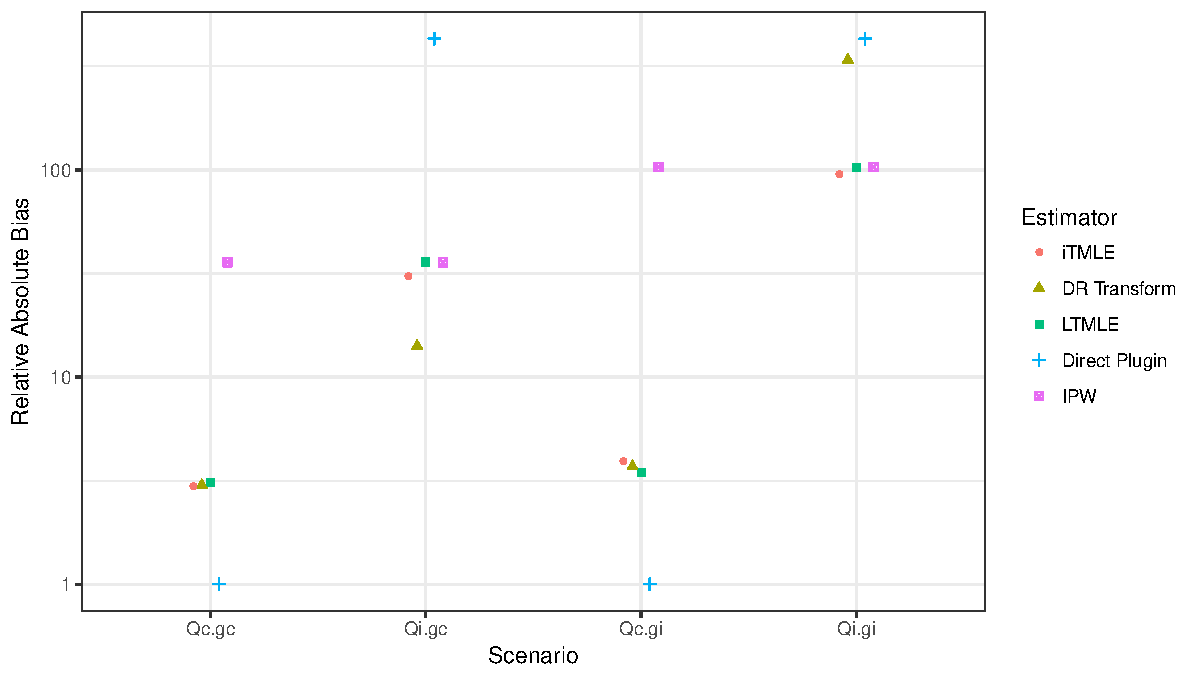
\includegraphics[width=.7\linewidth]{figure/plot-ggplot_bias_t3-1} 

}

\caption[Relative absolute bias for $\hat{Q}_0$ in simulation scenario 1 with 3 time points]{Relative absolute bias for $\hat{Q}_0$ in simulation scenario 1 with 3 time points.}\label{fig:ggplot.bias.t3}
\end{figure}


\end{knitrout}

% out.height = ".5\\linewidth",
\begin{knitrout}
\definecolor{shadecolor}{rgb}{0.969, 0.969, 0.969}\color{fgcolor}\begin{figure}[H]

{\centering 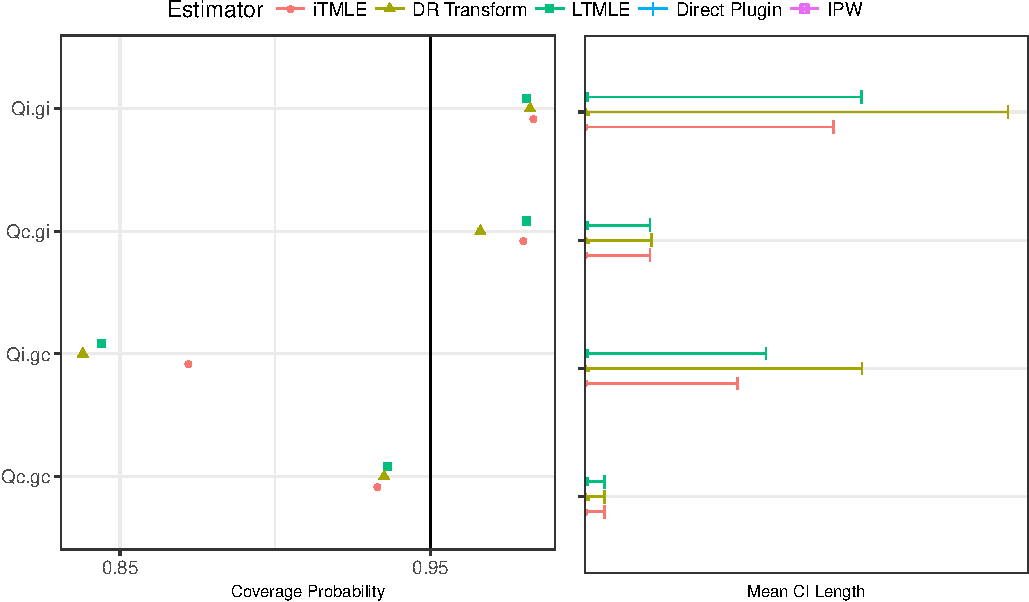
\includegraphics[width=.9\linewidth]{figure/plot-ggplot_CIcov_CIlen_t3-1} 

}

\caption[Coverage (left panel) and mean length (right panel) of the two-sided 95\% CIs for $Q_0$ in simulation scenario 1]{Coverage (left panel) and mean length (right panel) of the two-sided 95\% CIs for $Q_0$ in simulation scenario 1.}\label{fig:ggplot.CIcov.CIlen.t3}
\end{figure}


\end{knitrout}



\clearpage


%latex.default(restab, file = "", where = "H", caption.loc = "bottom",     caption = "Simulation scenario 1. Relative absolute bias for estimation of $Q_0$, over 3 time points and $n$=500.",     label = "tab1", booktabs = TRUE, landscape = FALSE, col.just = c("l",         "r"), size = "tiny")%
\begin{table}[H]
{\tiny
\begin{center}
\begin{tabular}{ll}
\toprule
\multicolumn{1}{l}{restab}&\multicolumn{1}{c}{Relative Bias}\tabularnewline
\midrule
Qc.gc.sdr&$  2.98$\tabularnewline
Qc.gc.drtrans&$  3.01$\tabularnewline
Qc.gc.tmle&$  3.11$\tabularnewline
Qc.gc.gcomp&$  1.00$\tabularnewline
Qc.gc.ipw&$ 35.84$\tabularnewline
Qi.gc.sdr&$ 30.80$\tabularnewline
Qi.gc.drtrans&$ 14.15$\tabularnewline
Qi.gc.tmle&$ 35.93$\tabularnewline
Qi.gc.gcomp&$430.36$\tabularnewline
Qi.gc.ipw&$ 35.84$\tabularnewline
Qc.gi.sdr&$  3.94$\tabularnewline
Qc.gi.drtrans&$  3.71$\tabularnewline
Qc.gi.tmle&$  3.46$\tabularnewline
Qc.gi.gcomp&$  1.00$\tabularnewline
Qc.gi.ipw&$103.31$\tabularnewline
Qi.gi.sdr&$ 95.58$\tabularnewline
Qi.gi.drtrans&$340.11$\tabularnewline
Qi.gi.tmle&$103.22$\tabularnewline
Qi.gi.gcomp&$430.36$\tabularnewline
Qi.gi.ipw&$103.31$\tabularnewline
\bottomrule
\end{tabular}

\caption{Simulation scenario 1. Relative absolute bias for estimation of $Q_0$, over 3 time points and $n$=500.\label{tab1}}\end{center}}

\end{table}



%latex.default(restab, file = "", where = "H", caption.loc = "bottom",     caption = "Simulation scenario 1. Relative MSE for estimation of $Q_1$, over 3 time points and $n$=500.",     label = "tab2", booktabs = TRUE, landscape = FALSE, col.just = c("l",         "r"), size = "tiny")%
\begin{table}[H]
{\tiny
\begin{center}
\begin{tabular}{ll}
\toprule
\multicolumn{1}{l}{restab}&\multicolumn{1}{c}{Relative MSE}\tabularnewline
\midrule
Qc.gc.sdr&$ 1.23$\tabularnewline
Qc.gc.drtrans&$ 1.47$\tabularnewline
Qc.gc.tmle&$ 1.21$\tabularnewline
Qc.gc.gcomp&$ 1.00$\tabularnewline
Qi.gc.sdr&$ 4.62$\tabularnewline
Qi.gc.drtrans&$12.54$\tabularnewline
Qi.gc.tmle&$12.18$\tabularnewline
Qi.gc.gcomp&$36.68$\tabularnewline
Qc.gi.sdr&$ 1.24$\tabularnewline
Qc.gi.drtrans&$ 1.71$\tabularnewline
Qc.gi.tmle&$ 1.21$\tabularnewline
Qc.gi.gcomp&$ 1.00$\tabularnewline
Qi.gi.sdr&$ 6.85$\tabularnewline
Qi.gi.drtrans&$34.52$\tabularnewline
Qi.gi.tmle&$14.19$\tabularnewline
Qi.gi.gcomp&$36.68$\tabularnewline
\bottomrule
\end{tabular}

\caption{Simulation scenario 1. Relative MSE for estimation of $Q_1$, over 3 time points and $n$=500.\label{tab2}}\end{center}}

\end{table}



%latex.default(restab, file = "", where = "H", caption.loc = "bottom",     caption = "Simulation scenario 1. Coverage of 95\\% CIs for $Q_0$, over 3 time points and $n$=500.",     booktabs = TRUE, landscape = FALSE, col.just = c("l", "r"),     size = "tiny")%
\begin{table}[H]
{\tiny
\begin{center}
\begin{tabular}{ll}
\toprule
\multicolumn{1}{l}{restab}&\multicolumn{1}{c}{Coverage prob.}\tabularnewline
\midrule
Qc.gc.sdr&$0.933$\tabularnewline
Qc.gc.drtrans&$0.935$\tabularnewline
Qc.gc.tmle&$0.936$\tabularnewline
Qc.gc.gcomp&$$\tabularnewline
Qi.gc.sdr&$0.872$\tabularnewline
Qi.gc.drtrans&$0.838$\tabularnewline
Qi.gc.tmle&$0.844$\tabularnewline
Qi.gc.gcomp&$$\tabularnewline
Qc.gi.sdr&$0.980$\tabularnewline
Qc.gi.drtrans&$0.966$\tabularnewline
Qc.gi.tmle&$0.981$\tabularnewline
Qc.gi.gcomp&$$\tabularnewline
Qi.gi.sdr&$0.983$\tabularnewline
Qi.gi.drtrans&$0.982$\tabularnewline
Qi.gi.tmle&$0.981$\tabularnewline
Qi.gi.gcomp&$$\tabularnewline
\bottomrule
\end{tabular}

\caption{Simulation scenario 1. Coverage of 95\% CIs for $Q_0$, over 3 time points and $n$=500.\label{restab}}\end{center}}

\end{table}


\clearpage

Data generating distribution for simulation scenario 1.

\begin{knitrout}
\definecolor{shadecolor}{rgb}{0.969, 0.969, 0.969}\color{fgcolor}\begin{kframe}
\begin{alltt}
\hlkwd{require}\hlstd{(}\hlstr{"simcausal"}\hlstd{)}
\hlstd{D} \hlkwb{<-} \hlkwd{DAG.empty}\hlstd{()} \hlopt{+}
    \hlkwd{node}\hlstd{(}\hlstr{"L"}\hlstd{,} \hlkwc{t} \hlstd{=} \hlnum{0}\hlstd{,} \hlkwc{distr} \hlstd{=} \hlstr{"rnorm"}\hlstd{)} \hlopt{+}
    \hlkwd{node}\hlstd{(}\hlstr{"A"}\hlstd{,} \hlkwc{t} \hlstd{=} \hlnum{0}\hlstd{,} \hlkwc{distr} \hlstd{=} \hlstr{"rbern"}\hlstd{,} \hlkwc{prob} \hlstd{=} \hlkwd{plogis}\hlstd{(L[}\hlnum{0}\hlstd{]))} \hlopt{+}
    \hlkwd{node}\hlstd{(}\hlstr{"Y"}\hlstd{,} \hlkwc{t} \hlstd{=} \hlnum{0}\hlstd{,} \hlkwc{distr} \hlstd{=} \hlstr{"rconst"}\hlstd{,} \hlkwc{const} \hlstd{=} \hlnum{0}\hlstd{)} \hlopt{+}
    \hlkwd{node}\hlstd{(}\hlstr{"L"}\hlstd{,} \hlkwc{t} \hlstd{=} \hlnum{1}\hlstd{,} \hlkwc{distr} \hlstd{=} \hlstr{"rnorm"}\hlstd{)} \hlopt{+}
    \hlkwd{node}\hlstd{(}\hlstr{"A"}\hlstd{,} \hlkwc{t} \hlstd{=} \hlnum{1}\hlstd{,} \hlkwc{distr} \hlstd{=} \hlstr{"rbern"}\hlstd{,} \hlkwc{prob} \hlstd{=} \hlkwd{plogis}\hlstd{(L[}\hlnum{1}\hlstd{]} \hlopt{+} \hlstd{A[}\hlnum{0}\hlstd{]))} \hlopt{+}
    \hlkwd{node}\hlstd{(}\hlstr{"Y"}\hlstd{,} \hlkwc{t} \hlstd{=} \hlnum{1}\hlstd{,} \hlkwc{distr} \hlstd{=} \hlstr{"rconst"}\hlstd{,} \hlkwc{const} \hlstd{=} \hlnum{0}\hlstd{)} \hlopt{+}
    \hlkwd{node}\hlstd{(}\hlstr{"L"}\hlstd{,} \hlkwc{t} \hlstd{=} \hlnum{2}\hlstd{,} \hlkwc{distr} \hlstd{=} \hlstr{"rnorm"}\hlstd{,} \hlkwc{mean} \hlstd{= L[}\hlnum{0}\hlstd{]}\hlopt{*}\hlstd{A[}\hlnum{1}\hlstd{]} \hlopt{+} \hlstd{A[}\hlnum{0}\hlstd{]}\hlopt{*}\hlstd{L[}\hlnum{1}\hlstd{]} \hlopt{+} \hlstd{L[}\hlnum{1}\hlstd{]}\hlopt{*}\hlstd{A[}\hlnum{1}\hlstd{])} \hlopt{+}
    \hlkwd{node}\hlstd{(}\hlstr{"A"}\hlstd{,} \hlkwc{t} \hlstd{=} \hlnum{2}\hlstd{,} \hlkwc{distr} \hlstd{=} \hlstr{"rbern"}\hlstd{,} \hlkwc{prob} \hlstd{=} \hlkwd{plogis}\hlstd{(L[}\hlnum{2}\hlstd{]} \hlopt{+} \hlstd{A[}\hlnum{1}\hlstd{]))} \hlopt{+}
    \hlkwd{node}\hlstd{(}\hlstr{"Y"}\hlstd{,} \hlkwc{t} \hlstd{=} \hlnum{2}\hlstd{,} \hlkwc{distr} \hlstd{=} \hlstr{"rbern"}\hlstd{,} \hlkwc{prob} \hlstd{=} \hlkwd{plogis}\hlstd{(L[}\hlnum{1}\hlstd{]}\hlopt{*}\hlstd{A[}\hlnum{2}\hlstd{]} \hlopt{+} \hlstd{A[}\hlnum{1}\hlstd{]}\hlopt{*}\hlstd{L[}\hlnum{2}\hlstd{]} \hlopt{+} \hlstd{L[}\hlnum{2}\hlstd{]}\hlopt{*}\hlstd{A[}\hlnum{2}\hlstd{]))}
\end{alltt}
\end{kframe}
\end{knitrout}

Model specification for simulation scenario 1.

\begin{knitrout}
\definecolor{shadecolor}{rgb}{0.969, 0.969, 0.969}\color{fgcolor}\begin{kframe}
\begin{alltt}
\hlstd{nsims} \hlkwb{<-} \hlnum{500}
\hlstd{nsamp} \hlkwb{<-} \hlnum{500}
\hlstd{tvals} \hlkwb{<-} \hlnum{2}
\hlcom{## g model (same across all time-points):}
\hlstd{gform.c} \hlkwb{<-} \hlstr{"A ~ L + Atm1"}
\hlstd{gform.i} \hlkwb{<-} \hlstr{"A ~ L"}
\hlcom{# Q models}
\hlstd{Qforms.c} \hlkwb{<-} \hlkwd{c}\hlstd{(}\hlstr{"Qkplus1 ~ L"}\hlstd{,}
              \hlstr{"Qkplus1 ~ A0L1 + L0A0 + L + A + Atm1 + Ltm1"}\hlstd{,}
              \hlstr{"Qkplus1 ~ A0L1 + L0A0 + L + A + Atm1 + Ltm1"}\hlstd{)}
\hlstd{Qinteract.c} \hlkwb{<-} \hlkwd{list}\hlstd{(}\hlkwd{c}\hlstd{(}\hlstr{"A"}\hlstd{,} \hlstr{"L"}\hlstd{),} \hlkwd{c}\hlstd{(}\hlstr{"A"}\hlstd{,} \hlstr{"Ltm1"}\hlstd{))}
\hlstd{Qforms.i} \hlkwb{<-} \hlkwd{c}\hlstd{(}\hlstr{"Qkplus1 ~ L"}\hlstd{,} \hlstr{"Qkplus1 ~ Atm1"}\hlstd{,} \hlstr{"Qkplus1 ~ Atm1"}\hlstd{)}
\hlstd{Qinteract.i} \hlkwb{<-} \hlkwa{NULL}
\end{alltt}
\end{kframe}
\end{knitrout}

\clearpage
\subsection{Demonstrating SDR property. Simulation scenario 2 with 5 time-points.}

\begin{knitrout}
\definecolor{shadecolor}{rgb}{0.969, 0.969, 0.969}\color{fgcolor}\begin{kframe}
\begin{alltt}
\hlkwd{load}\hlstd{(}\hlstr{"/Users/olegsofrygin/GoogleDrive/Alex_SDR/sims/sims_final_04_20_17/sim2_results_t4.Rd"}\hlstd{)}
\hlkwd{print}\hlstd{(results[[}\hlstr{"res_name"}\hlstd{]])}
\end{alltt}
\begin{verbatim}
## [1] "results for E[Y_d(t)] for \bar{A}=1, t=4, N = 5000, nsims = 1000"
\end{verbatim}
\end{kframe}
\end{knitrout}

\begin{knitrout}
\definecolor{shadecolor}{rgb}{0.969, 0.969, 0.969}\color{fgcolor}\begin{figure}[H]

{\centering 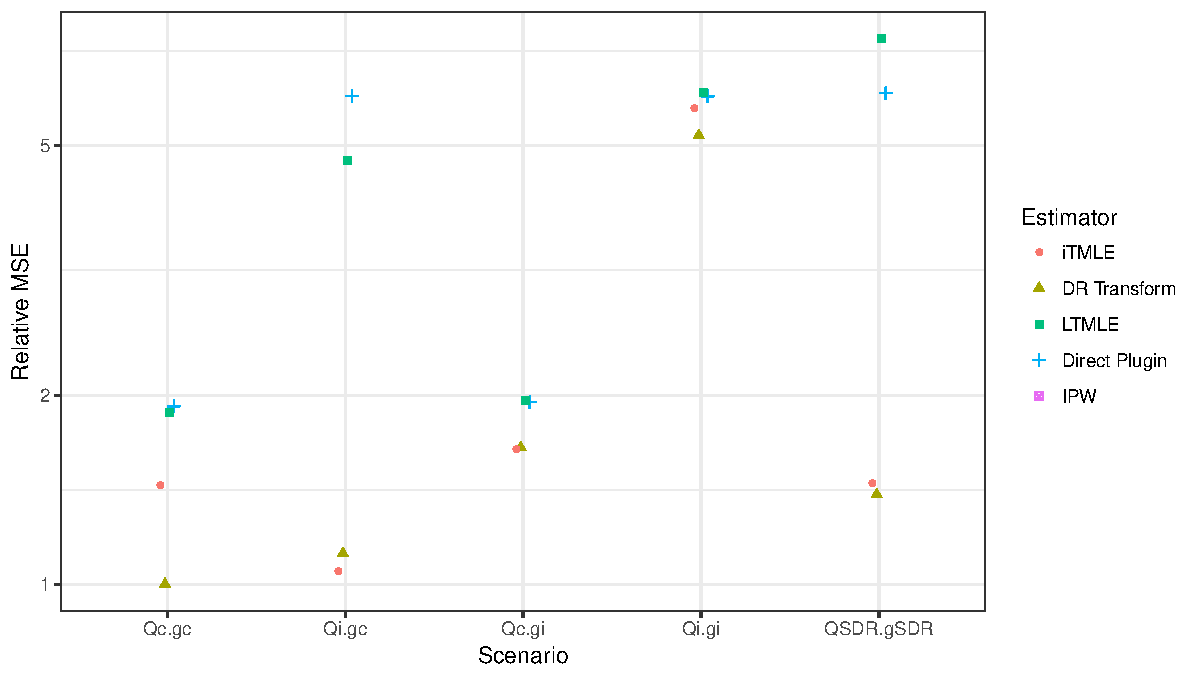
\includegraphics[width=.7\linewidth]{figure/plot-ggplot_MSE_t5-1} 

}

\caption[Relative MSE for $\hat{Q}_1$ in simulation scenario 2 with 5 time points]{Relative MSE for $\hat{Q}_1$ in simulation scenario 2 with 5 time points.}\label{fig:ggplot.MSE.t5}
\end{figure}


\end{knitrout}

\begin{knitrout}
\definecolor{shadecolor}{rgb}{0.969, 0.969, 0.969}\color{fgcolor}\begin{figure}[H]

{\centering 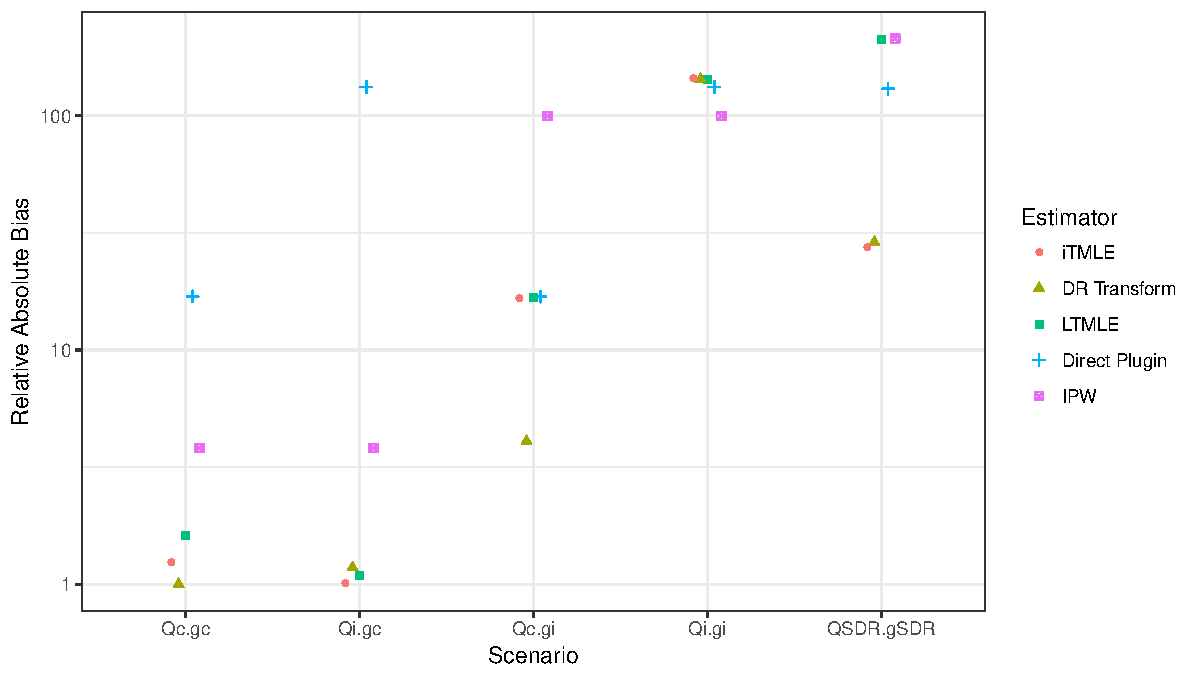
\includegraphics[width=.7\linewidth]{figure/plot-ggplot_bias_t5-1} 

}

\caption[Relative absolute bias for $\hat{Q}_0$ in simulation scenario 2 with 5 time points]{Relative absolute bias for $\hat{Q}_0$ in simulation scenario 2 with 5 time points.}\label{fig:ggplot.bias.t5}
\end{figure}


\end{knitrout}

\begin{knitrout}
\definecolor{shadecolor}{rgb}{0.969, 0.969, 0.969}\color{fgcolor}\begin{figure}[H]

{\centering 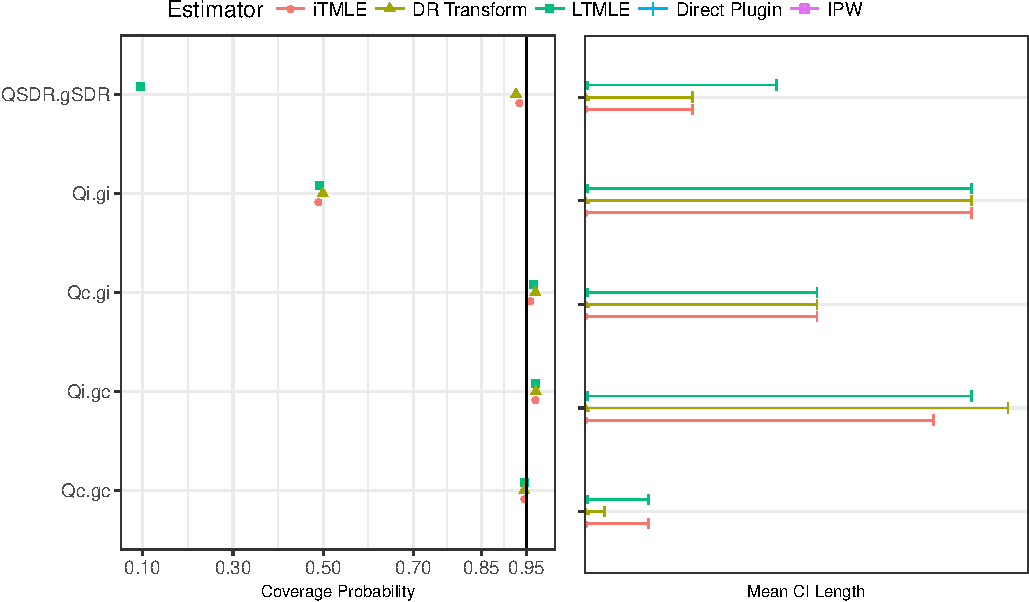
\includegraphics[width=.9\linewidth]{figure/plot-ggplot_CIcov_CIlen_t5-1} 

}

\caption[Coverage (left panel) and mean length (right panel) of the two-sided 95\% CIs for $Q_0$ in simulation scenario 2]{Coverage (left panel) and mean length (right panel) of the two-sided 95\% CIs for $Q_0$ in simulation scenario 2.}\label{fig:ggplot.CIcov.CIlen.t5}
\end{figure}


\end{knitrout}



\clearpage


%latex.default(restab, file = "", where = "H", caption.loc = "bottom",     caption = "Simulation scenario 2. Relative absolute bias for estimation of $Q_0$, over 5 time points and $n$=5,000.",     label = "tab1", booktabs = TRUE, landscape = FALSE, col.just = c("l",         "r"), size = "tiny")%
\begin{table}[H]
{\tiny
\begin{center}
\begin{tabular}{ll}
\toprule
\multicolumn{1}{l}{restab}&\multicolumn{1}{c}{Relative Bias}\tabularnewline
\midrule
Qc.gc.sdr&$  1.24$\tabularnewline
Qc.gc.drtrans&$  1.00$\tabularnewline
Qc.gc.tmle&$  1.61$\tabularnewline
Qc.gc.gcomp&$ 16.93$\tabularnewline
Qc.gc.ipw&$  3.82$\tabularnewline
Qi.gc.sdr&$  1.01$\tabularnewline
Qi.gc.drtrans&$  1.18$\tabularnewline
Qi.gc.tmle&$  1.09$\tabularnewline
Qi.gc.gcomp&$132.82$\tabularnewline
Qi.gc.ipw&$  3.82$\tabularnewline
Qc.gi.sdr&$ 16.71$\tabularnewline
Qc.gi.drtrans&$  4.08$\tabularnewline
Qc.gi.tmle&$ 16.74$\tabularnewline
Qc.gi.gcomp&$ 16.91$\tabularnewline
Qc.gi.ipw&$ 99.97$\tabularnewline
Qi.gi.sdr&$144.25$\tabularnewline
Qi.gi.drtrans&$143.26$\tabularnewline
Qi.gi.tmle&$143.12$\tabularnewline
Qi.gi.gcomp&$132.70$\tabularnewline
Qi.gi.ipw&$ 99.97$\tabularnewline
QSDR.gSDR.sdr&$ 27.60$\tabularnewline
QSDR.gSDR.drtrans&$ 28.89$\tabularnewline
QSDR.gSDR.tmle&$211.07$\tabularnewline
QSDR.gSDR.gcomp&$130.58$\tabularnewline
QSDR.gSDR.ipw&$213.37$\tabularnewline
\bottomrule
\end{tabular}

\caption{Simulation scenario 2. Relative absolute bias for estimation of $Q_0$, over 5 time points and $n$=5,000.\label{tab1}}\end{center}}

\end{table}



%latex.default(restab, file = "", where = "H", caption.loc = "bottom",     caption = "Simulation scenario 2. Relative MSE for estimation of $Q_1$, over 5 time points and $n$=5,000.",     label = "tab2", booktabs = TRUE, landscape = FALSE, col.just = c("l",         "r"), size = "tiny")%
\begin{table}[H]
{\tiny
\begin{center}
\begin{tabular}{ll}
\toprule
\multicolumn{1}{l}{restab}&\multicolumn{1}{c}{Relative MSE}\tabularnewline
\midrule
Qc.gc.sdr&$1.44$\tabularnewline
Qc.gc.drtrans&$1.00$\tabularnewline
Qc.gc.tmle&$1.88$\tabularnewline
Qc.gc.gcomp&$1.92$\tabularnewline
Qi.gc.sdr&$1.05$\tabularnewline
Qi.gc.drtrans&$1.12$\tabularnewline
Qi.gc.tmle&$4.74$\tabularnewline
Qi.gc.gcomp&$6.00$\tabularnewline
Qc.gi.sdr&$1.64$\tabularnewline
Qc.gi.drtrans&$1.65$\tabularnewline
Qc.gi.tmle&$1.96$\tabularnewline
Qc.gi.gcomp&$1.95$\tabularnewline
Qi.gi.sdr&$5.73$\tabularnewline
Qi.gi.drtrans&$5.19$\tabularnewline
Qi.gi.tmle&$6.08$\tabularnewline
Qi.gi.gcomp&$5.99$\tabularnewline
QSDR.gSDR.sdr&$1.45$\tabularnewline
QSDR.gSDR.drtrans&$1.39$\tabularnewline
QSDR.gSDR.tmle&$7.40$\tabularnewline
QSDR.gSDR.gcomp&$6.06$\tabularnewline
\bottomrule
\end{tabular}

\caption{Simulation scenario 2. Relative MSE for estimation of $Q_1$, over 5 time points and $n$=5,000.\label{tab2}}\end{center}}

\end{table}



%latex.default(restab, file = "", where = "H", caption.loc = "bottom",     caption = "Simulation scenario 2. Coverage of 95\\% CIs for $Q_0$, over 5 time points and $n$=5,000.",     booktabs = TRUE, landscape = FALSE, col.just = c("l", "r"),     size = "tiny")%
\begin{table}[H]
{\tiny
\begin{center}
\begin{tabular}{ll}
\toprule
\multicolumn{1}{l}{restab}&\multicolumn{1}{c}{Coverage prob.}\tabularnewline
\midrule
Qc.gc.sdr&$0.946$\tabularnewline
Qc.gc.drtrans&$0.945$\tabularnewline
Qc.gc.tmle&$0.945$\tabularnewline
Qc.gc.gcomp&$$\tabularnewline
Qi.gc.sdr&$0.970$\tabularnewline
Qi.gc.drtrans&$0.971$\tabularnewline
Qi.gc.tmle&$0.971$\tabularnewline
Qi.gc.gcomp&$$\tabularnewline
Qc.gi.sdr&$0.958$\tabularnewline
Qc.gi.drtrans&$0.970$\tabularnewline
Qc.gi.tmle&$0.965$\tabularnewline
Qc.gi.gcomp&$$\tabularnewline
Qi.gi.sdr&$0.489$\tabularnewline
Qi.gi.drtrans&$0.499$\tabularnewline
Qi.gi.tmle&$0.492$\tabularnewline
Qi.gi.gcomp&$$\tabularnewline
QSDR.gSDR.sdr&$0.935$\tabularnewline
QSDR.gSDR.drtrans&$0.927$\tabularnewline
QSDR.gSDR.tmle&$0.095$\tabularnewline
QSDR.gSDR.gcomp&$$\tabularnewline
\bottomrule
\end{tabular}

\caption{Simulation scenario 2. Coverage of 95\% CIs for $Q_0$, over 5 time points and $n$=5,000.\label{restab}}\end{center}}

\end{table}


\clearpage

Data generating distribution for simulation scenario 2.

\begin{knitrout}
\definecolor{shadecolor}{rgb}{0.969, 0.969, 0.969}\color{fgcolor}\begin{kframe}
\begin{alltt}
\hlstd{nsims} \hlkwb{<-} \hlnum{500}
\hlstd{nsamp} \hlkwb{<-} \hlnum{5000}
\hlstd{tvals} \hlkwb{<-} \hlnum{4}
\hlkwd{require}\hlstd{(}\hlstr{"simcausal"}\hlstd{)}
\hlstd{D} \hlkwb{<-} \hlkwd{DAG.empty}\hlstd{()} \hlopt{+}
    \hlkwd{node}\hlstd{(}\hlstr{"UL"}\hlstd{,}    \hlkwc{t} \hlstd{=} \hlnum{0}\hlstd{,} \hlkwc{distr} \hlstd{=} \hlstr{"rnorm"}\hlstd{)} \hlopt{+}
    \hlkwd{node}\hlstd{(}\hlstr{"W"}\hlstd{,}     \hlkwc{t} \hlstd{=} \hlnum{0}\hlstd{,} \hlkwc{distr} \hlstd{=} \hlstr{"rnorm"}\hlstd{,} \hlkwc{mean} \hlstd{=} \hlnum{0}\hlstd{)} \hlopt{+}
    \hlkwd{node}\hlstd{(}\hlstr{"L"}\hlstd{,}     \hlkwc{t} \hlstd{=} \hlnum{0}\hlstd{,} \hlkwc{distr} \hlstd{=} \hlstr{"rconst"}\hlstd{,} \hlkwc{const} \hlstd{=} \hlkwd{abs}\hlstd{(UL[t]))} \hlopt{+}
    \hlkwd{node}\hlstd{(}\hlstr{"phiRsk"}\hlstd{,} \hlkwc{t} \hlstd{=} \hlnum{0}\hlstd{,} \hlkwc{distr} \hlstd{=} \hlstr{"rconst"}\hlstd{,} \hlkwc{const} \hlstd{= L[}\hlnum{0}\hlstd{])} \hlopt{+}
    \hlkwd{node}\hlstd{(}\hlstr{"hiRsk"}\hlstd{,} \hlkwc{t} \hlstd{=} \hlnum{0}\hlstd{,} \hlkwc{distr} \hlstd{=} \hlstr{"rconst"}\hlstd{,} \hlkwc{const} \hlstd{=} \hlkwd{plogis}\hlstd{(phiRsk[t])} \hlopt{>} \hlnum{0.8}\hlstd{)} \hlopt{+}
    \hlkwd{node}\hlstd{(}\hlstr{"A"}\hlstd{,}     \hlkwc{t} \hlstd{=} \hlnum{0}\hlstd{,} \hlkwc{distr} \hlstd{=} \hlstr{"rbern"}\hlstd{,} \hlkwc{prob} \hlstd{=} \hlkwd{plogis}\hlstd{(L[}\hlnum{0}\hlstd{]))} \hlopt{+}
    \hlkwd{node}\hlstd{(}\hlstr{"Y"}\hlstd{,}     \hlkwc{t} \hlstd{=} \hlnum{0}\hlstd{,} \hlkwc{distr} \hlstd{=} \hlstr{"rconst"}\hlstd{,} \hlkwc{const} \hlstd{=} \hlnum{0}\hlstd{)} \hlopt{+}

    \hlkwd{node}\hlstd{(}\hlstr{"UL"}\hlstd{,}\hlkwc{t} \hlstd{=} \hlnum{1}\hlstd{,} \hlkwc{distr} \hlstd{=} \hlstr{"rnorm"}\hlstd{)} \hlopt{+}
    \hlkwd{node}\hlstd{(}\hlstr{"L"}\hlstd{,} \hlkwc{t} \hlstd{=} \hlnum{1}\hlstd{,} \hlkwc{distr} \hlstd{=} \hlstr{"rconst"}\hlstd{,} \hlkwc{const} \hlstd{=} \hlkwd{abs}\hlstd{(UL[t]))} \hlopt{+}
    \hlkwd{node}\hlstd{(}\hlstr{"phiRsk"}\hlstd{,} \hlkwc{t} \hlstd{=} \hlnum{1}\hlstd{,} \hlkwc{distr} \hlstd{=} \hlstr{"rconst"}\hlstd{,} \hlkwc{const} \hlstd{=} \hlopt{-}\hlnum{2} \hlopt{+} \hlnum{0.5}\hlopt{*}\hlstd{L[t}\hlopt{-}\hlnum{1}\hlstd{]} \hlopt{+} \hlnum{0.5}\hlopt{*}\hlnum{2}\hlopt{*}\hlstd{L[t])} \hlopt{+}
    \hlkwd{node}\hlstd{(}\hlstr{"hiRsk"}\hlstd{,} \hlkwc{t} \hlstd{=} \hlnum{1}\hlstd{,} \hlkwc{distr} \hlstd{=} \hlstr{"rconst"}\hlstd{,} \hlkwc{const} \hlstd{=} \hlkwd{plogis}\hlstd{(phiRsk[t])} \hlopt{>} \hlnum{0.9}\hlstd{)} \hlopt{+}
    \hlkwd{node}\hlstd{(}\hlstr{"A"}\hlstd{,} \hlkwc{t} \hlstd{=} \hlnum{1}\hlstd{,} \hlkwc{distr} \hlstd{=} \hlstr{"rbern"}\hlstd{,} \hlkwc{prob} \hlstd{= A[t}\hlopt{-}\hlnum{1}\hlstd{]}\hlopt{*}\hlkwd{plogis}\hlstd{(}\hlnum{1.7} \hlopt{-} \hlnum{2.0}\hlopt{*}\hlstd{hiRsk[t]))} \hlopt{+}
    \hlkwd{node}\hlstd{(}\hlstr{"Y"}\hlstd{,} \hlkwc{t} \hlstd{=} \hlnum{1}\hlstd{,} \hlkwc{distr} \hlstd{=} \hlstr{"rbern"}\hlstd{,}
      \hlkwc{prob} \hlstd{=} \hlkwd{plogis}\hlstd{(}\hlopt{-}\hlnum{3} \hlopt{+} \hlnum{0.5}\hlopt{*}\hlstd{L[t}\hlopt{-}\hlnum{1}\hlstd{]}\hlopt{*}\hlstd{A[t]} \hlopt{+} \hlnum{0.5}\hlopt{*}\hlstd{A[t}\hlopt{-}\hlnum{1}\hlstd{]}\hlopt{*}\hlstd{L[t]} \hlopt{+} \hlnum{0.5}\hlopt{*}\hlstd{L[t]}\hlopt{*}\hlstd{A[t]))} \hlopt{+}

    \hlkwd{node}\hlstd{(}\hlstr{"UL"}\hlstd{,}\hlkwc{t} \hlstd{=} \hlnum{2}\hlstd{,} \hlkwc{distr} \hlstd{=} \hlstr{"rnorm"}\hlstd{,} \hlkwc{mean} \hlstd{= A[}\hlnum{0}\hlstd{]}\hlopt{*}\hlstd{L[}\hlnum{1}\hlstd{]} \hlopt{+} \hlstd{L[}\hlnum{1}\hlstd{]}\hlopt{*}\hlstd{A[}\hlnum{1}\hlstd{])} \hlopt{+}
    \hlkwd{node}\hlstd{(}\hlstr{"L"}\hlstd{,} \hlkwc{t} \hlstd{=} \hlnum{2}\hlstd{,} \hlkwc{distr} \hlstd{=} \hlstr{"rconst"}\hlstd{,} \hlkwc{const} \hlstd{=} \hlkwd{abs}\hlstd{(UL[t]))} \hlopt{+}
    \hlkwd{node}\hlstd{(}\hlstr{"phiRsk"}\hlstd{,} \hlkwc{t} \hlstd{=} \hlnum{2}\hlstd{,} \hlkwc{distr} \hlstd{=} \hlstr{"rconst"}\hlstd{,} \hlkwc{const} \hlstd{=} \hlopt{-}\hlnum{2} \hlopt{+} \hlnum{0.5}\hlopt{*}\hlstd{L[t}\hlopt{-}\hlnum{1}\hlstd{]} \hlopt{+} \hlnum{0.5}\hlopt{*}\hlnum{2}\hlopt{*}\hlstd{L[t])} \hlopt{+}
    \hlkwd{node}\hlstd{(}\hlstr{"hiRsk"}\hlstd{,} \hlkwc{t} \hlstd{=} \hlnum{2}\hlstd{,} \hlkwc{distr} \hlstd{=} \hlstr{"rconst"}\hlstd{,} \hlkwc{const} \hlstd{=} \hlkwd{plogis}\hlstd{(phiRsk[t])} \hlopt{>} \hlnum{0.85}\hlstd{)} \hlopt{+}
    \hlkwd{node}\hlstd{(}\hlstr{"A"}\hlstd{,} \hlkwc{t} \hlstd{=} \hlnum{2}\hlstd{,} \hlkwc{distr} \hlstd{=} \hlstr{"rbern"}\hlstd{,} \hlkwc{prob} \hlstd{= A[t}\hlopt{-}\hlnum{1}\hlstd{]}\hlopt{*}\hlkwd{plogis}\hlstd{(}\hlnum{1.7} \hlopt{-} \hlnum{2.0}\hlopt{*}\hlstd{hiRsk[t]))} \hlopt{+}
    \hlkwd{node}\hlstd{(}\hlstr{"Y"}\hlstd{,} \hlkwc{t} \hlstd{=} \hlnum{2}\hlstd{,} \hlkwc{distr} \hlstd{=} \hlstr{"rbern"}\hlstd{,}
      \hlkwc{prob} \hlstd{=} \hlkwd{plogis}\hlstd{(}\hlopt{-}\hlnum{3}\hlopt{*}\hlstd{Y[t}\hlopt{-}\hlnum{1}\hlstd{]} \hlopt{+} \hlnum{0.5}\hlopt{*}\hlstd{L[t}\hlopt{-}\hlnum{1}\hlstd{]}\hlopt{*}\hlstd{A[t]} \hlopt{+} \hlnum{0.5}\hlopt{*}\hlstd{A[t}\hlopt{-}\hlnum{1}\hlstd{]}\hlopt{*}\hlstd{L[t]} \hlopt{+} \hlnum{0.5}\hlopt{*}\hlstd{L[t]}\hlopt{*}\hlstd{A[t]))} \hlopt{+}

    \hlkwd{node}\hlstd{(}\hlstr{"UL"}\hlstd{,}\hlkwc{t} \hlstd{=} \hlnum{3}\hlstd{,} \hlkwc{distr} \hlstd{=} \hlstr{"rnorm"}\hlstd{,} \hlkwc{mean} \hlstd{= L[}\hlnum{1}\hlstd{]} \hlopt{*} \hlstd{A[t}\hlopt{-}\hlnum{1}\hlstd{]} \hlopt{+} \hlstd{A[}\hlnum{1}\hlstd{]}\hlopt{*}\hlstd{L[t}\hlopt{-}\hlnum{1}\hlstd{]} \hlopt{+} \hlstd{L[t}\hlopt{-}\hlnum{1}\hlstd{]}\hlopt{*}\hlstd{A[t}\hlopt{-}\hlnum{1}\hlstd{])} \hlopt{+}
    \hlkwd{node}\hlstd{(}\hlstr{"L"}\hlstd{,} \hlkwc{t} \hlstd{=} \hlnum{3}\hlstd{,} \hlkwc{distr} \hlstd{=} \hlstr{"rconst"}\hlstd{,} \hlkwc{const} \hlstd{=} \hlkwd{abs}\hlstd{(UL[t]))} \hlopt{+}
    \hlkwd{node}\hlstd{(}\hlstr{"phiRsk"}\hlstd{,} \hlkwc{t} \hlstd{=} \hlnum{3}\hlstd{,} \hlkwc{distr} \hlstd{=} \hlstr{"rconst"}\hlstd{,} \hlkwc{const} \hlstd{=} \hlopt{-}\hlnum{2} \hlopt{+} \hlnum{0.5}\hlopt{*}\hlstd{L[t}\hlopt{-}\hlnum{1}\hlstd{]} \hlopt{+} \hlnum{0.5}\hlopt{*}\hlnum{2}\hlopt{*}\hlstd{L[t])} \hlopt{+}
    \hlkwd{node}\hlstd{(}\hlstr{"hiRsk"}\hlstd{,} \hlkwc{t} \hlstd{=} \hlnum{3}\hlstd{,} \hlkwc{distr} \hlstd{=} \hlstr{"rconst"}\hlstd{,} \hlkwc{const} \hlstd{=} \hlkwd{plogis}\hlstd{(phiRsk[t])} \hlopt{>} \hlnum{0.80}\hlstd{)} \hlopt{+}
    \hlkwd{node}\hlstd{(}\hlstr{"A"}\hlstd{,} \hlkwc{t} \hlstd{=} \hlnum{3}\hlstd{,} \hlkwc{distr} \hlstd{=} \hlstr{"rbern"}\hlstd{,} \hlkwc{prob} \hlstd{= A[t}\hlopt{-}\hlnum{1}\hlstd{]}\hlopt{*}\hlkwd{plogis}\hlstd{(}\hlnum{1.7} \hlopt{-} \hlnum{2.0}\hlopt{*}\hlstd{hiRsk[t]))} \hlopt{+}
    \hlkwd{node}\hlstd{(}\hlstr{"Y"}\hlstd{,} \hlkwc{t} \hlstd{=} \hlnum{3}\hlstd{,} \hlkwc{distr} \hlstd{=} \hlstr{"rbern"}\hlstd{,}
      \hlkwc{prob} \hlstd{=} \hlkwd{plogis}\hlstd{(}\hlopt{-}\hlnum{3}\hlopt{*}\hlstd{Y[t}\hlopt{-}\hlnum{1}\hlstd{]} \hlopt{+} \hlnum{0.5}\hlopt{*}\hlstd{L[t}\hlopt{-}\hlnum{1}\hlstd{]}\hlopt{*}\hlstd{A[t]} \hlopt{+} \hlnum{0.5}\hlopt{*}\hlstd{A[t}\hlopt{-}\hlnum{1}\hlstd{]}\hlopt{*}\hlstd{L[t]} \hlopt{+} \hlnum{0.5}\hlopt{*}\hlstd{L[t]}\hlopt{*}\hlstd{A[t]))} \hlopt{+}

    \hlkwd{node}\hlstd{(}\hlstr{"UL"}\hlstd{,}\hlkwc{t} \hlstd{=} \hlnum{4}\hlstd{,} \hlkwc{distr} \hlstd{=} \hlstr{"rnorm"}\hlstd{,} \hlkwc{mean} \hlstd{= L[}\hlnum{1}\hlstd{]} \hlopt{*} \hlstd{A[t}\hlopt{-}\hlnum{1}\hlstd{]} \hlopt{+} \hlstd{A[}\hlnum{1}\hlstd{]}\hlopt{*}\hlstd{L[t}\hlopt{-}\hlnum{1}\hlstd{]} \hlopt{+} \hlstd{L[t}\hlopt{-}\hlnum{1}\hlstd{]}\hlopt{*}\hlstd{A[t}\hlopt{-}\hlnum{1}\hlstd{])} \hlopt{+}
    \hlkwd{node}\hlstd{(}\hlstr{"L"}\hlstd{,} \hlkwc{t} \hlstd{=} \hlnum{4}\hlstd{,} \hlkwc{distr} \hlstd{=} \hlstr{"rconst"}\hlstd{,} \hlkwc{const} \hlstd{=} \hlkwd{abs}\hlstd{(UL[t]))} \hlopt{+}
    \hlkwd{node}\hlstd{(}\hlstr{"phiRsk"}\hlstd{,} \hlkwc{t} \hlstd{=} \hlnum{4}\hlstd{,} \hlkwc{distr} \hlstd{=} \hlstr{"rconst"}\hlstd{,}
      \hlkwc{const} \hlstd{=} \hlopt{-}\hlnum{1} \hlopt{+} \hlnum{0.25}\hlopt{*}\hlstd{L[t}\hlopt{-}\hlnum{1}\hlstd{]} \hlopt{+} \hlnum{0.25}\hlopt{*}\hlnum{2}\hlopt{*}\hlstd{L[t]} \hlopt{-} \hlnum{0.1}\hlopt{*}\hlstd{L[t]}\hlopt{*}\hlstd{L[t}\hlopt{-}\hlnum{1}\hlstd{]} \hlopt{+} \hlnum{1.5}\hlopt{*}\hlstd{W[}\hlnum{0}\hlstd{]}\hlopt{*}\hlstd{L[t}\hlopt{-}\hlnum{1}\hlstd{])} \hlopt{+}
    \hlkwd{node}\hlstd{(}\hlstr{"hiRsk"}\hlstd{,} \hlkwc{t} \hlstd{=} \hlnum{4}\hlstd{,} \hlkwc{distr} \hlstd{=} \hlstr{"rconst"}\hlstd{,} \hlkwc{const} \hlstd{=} \hlkwd{plogis}\hlstd{(phiRsk[t])} \hlopt{>} \hlnum{0.80}\hlstd{)} \hlopt{+}
    \hlkwd{node}\hlstd{(}\hlstr{"A"}\hlstd{,} \hlkwc{t} \hlstd{=} \hlnum{4}\hlstd{,} \hlkwc{distr} \hlstd{=} \hlstr{"rbern"}\hlstd{,} \hlkwc{prob} \hlstd{= A[t}\hlopt{-}\hlnum{1}\hlstd{]}\hlopt{*}\hlkwd{plogis}\hlstd{(}\hlnum{2} \hlopt{-} \hlnum{2.0}\hlopt{*}\hlstd{hiRsk[t]))} \hlopt{+}
    \hlkwd{node}\hlstd{(}\hlstr{"Y"}\hlstd{,} \hlkwc{t} \hlstd{=} \hlnum{4}\hlstd{,} \hlkwc{distr} \hlstd{=} \hlstr{"rbern"}\hlstd{,}
      \hlkwc{prob} \hlstd{=} \hlkwd{plogis}\hlstd{(}\hlopt{-}\hlnum{1}\hlopt{*}\hlstd{Y[t}\hlopt{-}\hlnum{1}\hlstd{]} \hlopt{+} \hlstd{A[t]} \hlopt{+} \hlstd{phiRsk[t]}\hlopt{*}\hlstd{A[t]} \hlopt{+} \hlnum{0.20}\hlopt{*}\hlstd{A[t}\hlopt{-}\hlnum{1}\hlstd{]}\hlopt{*}\hlstd{L[t]) )}
\end{alltt}
\end{kframe}
\end{knitrout}

\clearpage
Model specification for simulation scenario 2.

\begin{knitrout}
\definecolor{shadecolor}{rgb}{0.969, 0.969, 0.969}\color{fgcolor}\begin{kframe}
\begin{alltt}
\hlcom{## g model (same across all time-points):}
\hlstd{gform.c} \hlkwb{<-} \hlkwd{c}\hlstd{(}\hlkwd{rep.int}\hlstd{(}\hlstr{"A ~ hiRsk + L + Atm1 + Ytm1"}\hlstd{, tvals),} \hlstr{"A ~ hiRsk + Atm1 + Ytm1"}\hlstd{)}
\hlstd{gform.i} \hlkwb{<-} \hlstr{"A ~ 1"}

\hlcom{## Q models:}
\hlstd{Qforms.c} \hlkwb{<-} \hlkwd{c}\hlstd{(}\hlstr{"Qkplus1 ~ L + W"}\hlstd{,}
              \hlstr{"Qkplus1 ~ L + Ltm1 + A + Atm1 + Ytm1 + W"}\hlstd{,}
              \hlstr{"Qkplus1 ~ L + Ltm1 + Ltm2 + A + Atm1 + Atm2 + Ytm1 + W"}\hlstd{,}
              \hlstr{"Qkplus1 ~ L + Ltm1 + Ltm2 + A + Atm1 + Atm2 + Ytm1 + W"}\hlstd{,}
              \hlstr{"Qkplus1 ~ L + Ltm1 + A + Atm1 + Ytm1 + W"}
              \hlstd{)}
\hlstd{Qinteract.c} \hlkwb{<-} \hlkwa{NULL}

\hlstd{Qforms.i} \hlkwb{<-} \hlkwd{c}\hlstd{(}\hlstr{"Qkplus1 ~ L + W"}\hlstd{,}
              \hlstr{"Qkplus1 ~ W"}\hlstd{,}
              \hlstr{"Qkplus1 ~ W"}\hlstd{,}
              \hlstr{"Qkplus1 ~ W"}\hlstd{,}
              \hlstr{"Qkplus1 ~ W"}\hlstd{)}
\hlstd{Qinteract.i} \hlkwb{<-} \hlkwa{NULL}

\hlcom{## g and Q model to demonstrate SDR property (only last g is correctly specified)}
\hlstd{gform.SDR} \hlkwb{<-} \hlkwd{c}\hlstd{(}\hlkwd{rep.int}\hlstd{(}\hlstr{"A ~ 1"}\hlstd{, tvals}\hlopt{-}\hlnum{1}\hlstd{),} \hlstr{"A ~ 1"}\hlstd{,} \hlstr{"A ~ hiRsk + Atm1 + Ytm1"}\hlstd{)}
\hlstd{Qforms.SDR} \hlkwb{<-} \hlkwd{c}\hlstd{(}\hlstr{"Qkplus1 ~ L + W"}\hlstd{,}
                \hlstr{"Qkplus1 ~ L + Ltm1 + A + Atm1 + Ytm1 + W"}\hlstd{,}
                \hlstr{"Qkplus1 ~ L + Ltm1 + A + Atm1 + Ytm1 + W"}\hlstd{,}
                \hlstr{"Qkplus1 ~ L + Ltm1 + A + Atm1 + Ytm1 + W"}\hlstd{,}
                \hlstr{"Qkplus1 ~ W"}\hlstd{)}
\hlstd{Qinteract.SDR} \hlkwb{<-} \hlkwa{NULL}
\end{alltt}
\end{kframe}
\end{knitrout}

\clearpage
\subsection{Combined results for simulation scenarios 1 and 2.}

\begin{knitrout}
\definecolor{shadecolor}{rgb}{0.969, 0.969, 0.969}\color{fgcolor}\begin{figure}[H]

{\centering 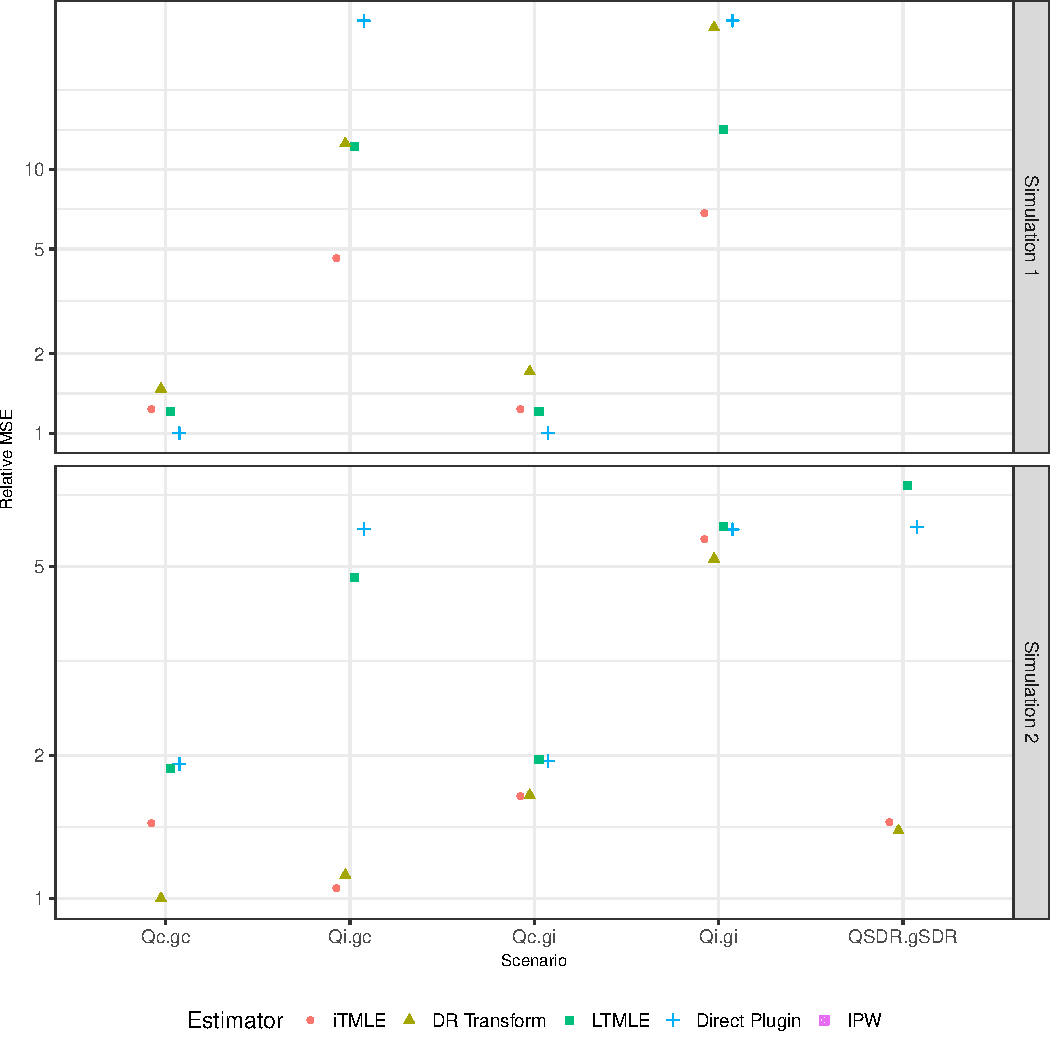
\includegraphics[width=.65\linewidth]{figure/plot-simres_all_MSE-1} 

}

\caption[Relative MSE for $\hat{Q}_1$ for simulation scenario 1 (top panel) and simulation scenario 2 (bottom panel)]{Relative MSE for $\hat{Q}_1$ for simulation scenario 1 (top panel) and simulation scenario 2 (bottom panel). Simulation 1 is based on longitudinal data with 3 time-points and $n$=500 observations. Simulation 2 is based on longitudinal data with 5 time-points and $n$=5,000 observations. The iTMLE and DR Transform typically outperform or perform comparably to both competitors.}\label{fig:simres.all.MSE}
\end{figure}


\end{knitrout}

\begin{knitrout}
\definecolor{shadecolor}{rgb}{0.969, 0.969, 0.969}\color{fgcolor}\begin{figure}[H]

{\centering 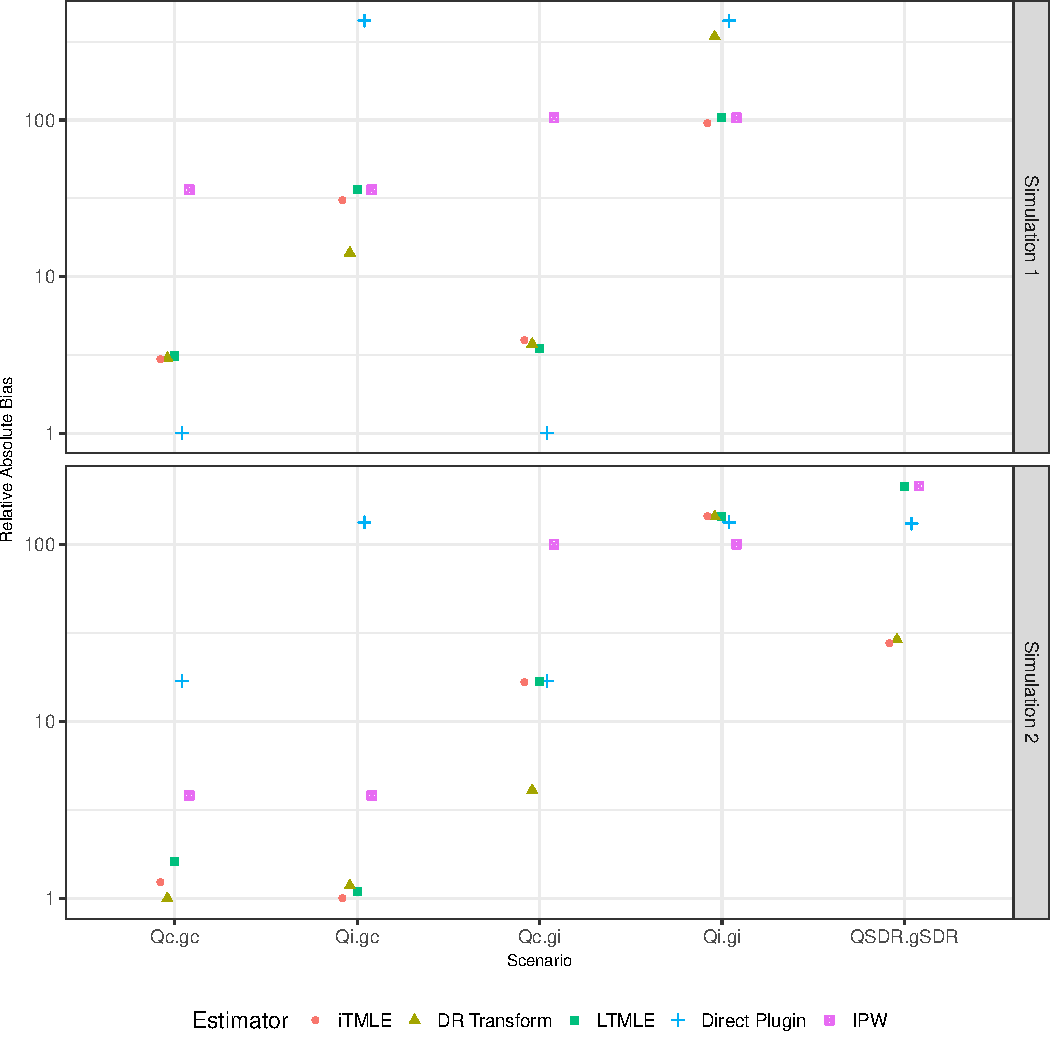
\includegraphics[width=.65\linewidth]{figure/plot-simres_all_BIAS-1} 

}

\caption{Relative absolute bias for $\hat{Q}_0$ for simulation scenario 1 (top panel) and simulation scenario 2 (bottom panel). Simulation 1 is based on longitudinal data with 3 time-points and $n$=500 observations. Simulation 2 is based on longitudinal data with 5 time-points and $n$=5,000 observations. The performance of LTMLE, iTMLE, and DR Transform is similar. The only exception for Simulation 1 is under \textit{Qi.gc}, where DR Transform outperforms other methods. The only exceptions for Simulation 2 are for \textit{Qc.gi}, where DR Transform outperforms other methods, and \textit{QSDR.gSDR}, where both SDR methods outperform LTMLE.}\label{fig:simres.all.BIAS}
\end{figure}


\end{knitrout}

\begin{knitrout}
\definecolor{shadecolor}{rgb}{0.969, 0.969, 0.969}\color{fgcolor}\begin{figure}[H]

{\centering 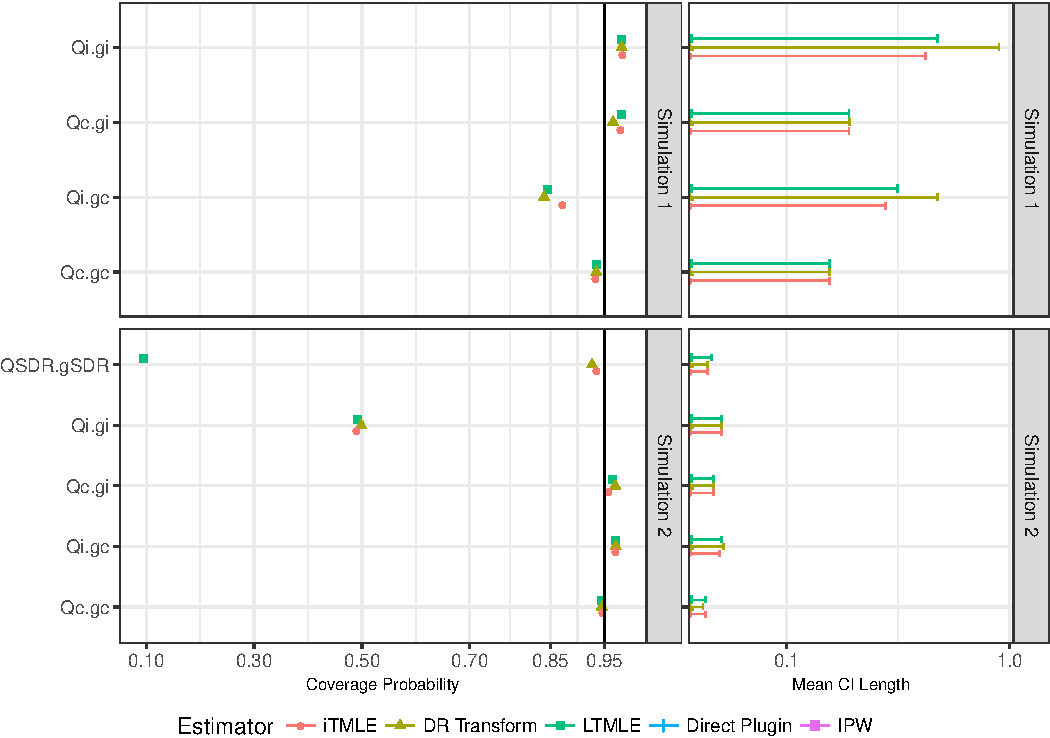
\includegraphics[width=.9\linewidth]{figure/plot-simres_all_coverCIlen-1} 

}

\caption{Coverage (left panels) and mean length (right panels) of the two-sided 95\% CIs for $Q_0$ in simulation scenario 1 (top panels) and simulation scenario 2 (bottom panels). Confidence interval coverage and width appear to be comparable between the two SDR methods and the LTMLE. The only exception is for the \textit{QSDR.gSDR} scenario, where the LTMLE has roughly 10\% coverage, whereas the SDR  approaches nearly achieve the nominal coverage level.}\label{fig:simres.all.coverCIlen}
\end{figure}


\end{knitrout}

\clearpage
\begin{knitrout}
\definecolor{shadecolor}{rgb}{0.969, 0.969, 0.969}\color{fgcolor}\begin{figure}

{\centering 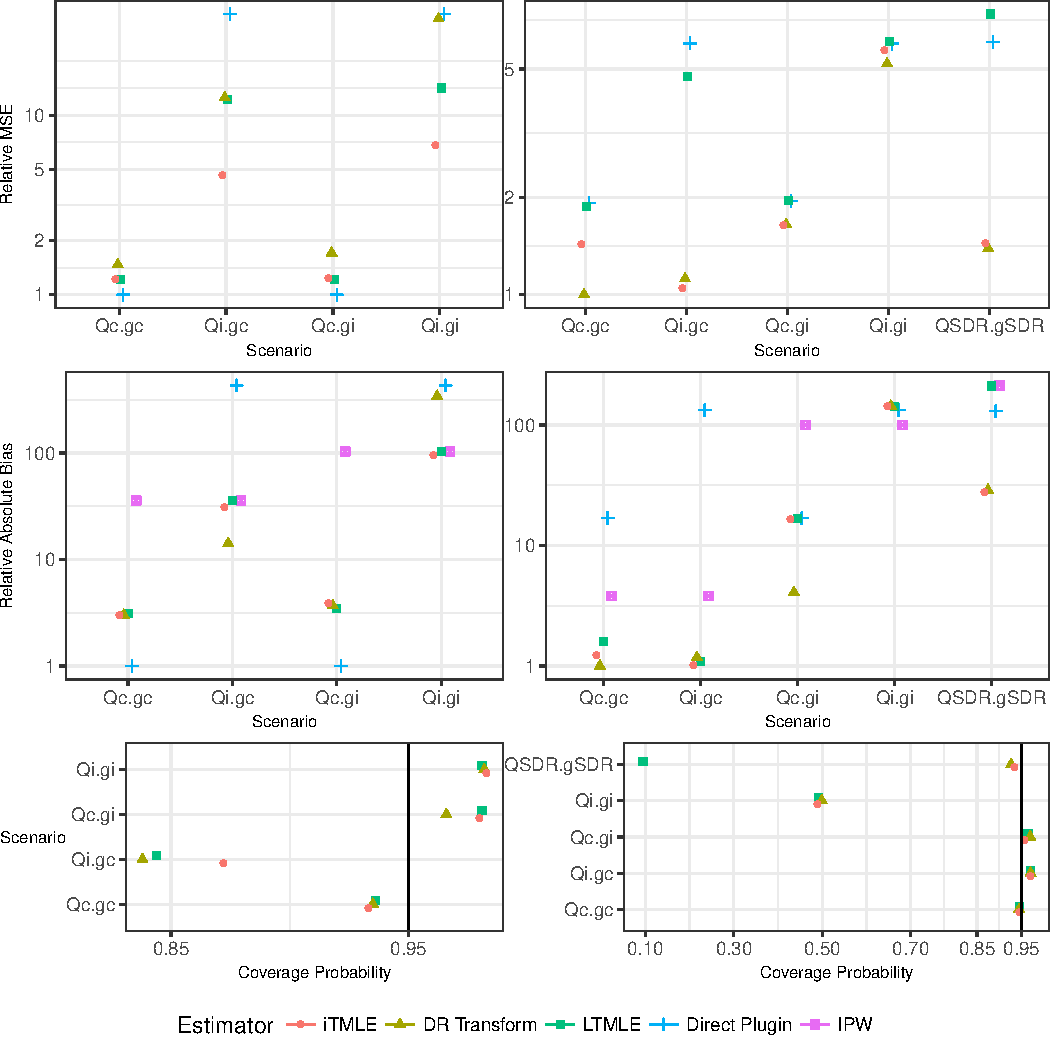
\includegraphics[width=\maxwidth]{figure/plot-ggplot_all-1} 

}

\caption[Top to bottom]{Top to bottom: MSE for estimation of $Q_1$, bias for estimation of $Q_0$ and 95\% CI coverage for estimation of $Q_0$. Left plot: simulation scenario 1. Right plot: simulation scenario 2.}\label{fig:ggplot.all}
\end{figure}


\end{knitrout}




\end{document}
